\documentclass[11pt,letterpaper]{article}

\usepackage[margin=0.95in]{geometry}
\usepackage{microtype}
\usepackage{graphicx}
\usepackage{booktabs}
\usepackage{xcolor}
\usepackage{hyperref}
\usepackage{caption}

\definecolor{accent}{HTML}{01696F}
\definecolor{accentdark}{HTML}{0C4E54}
\definecolor{muted}{HTML}{7A7974}

\hypersetup{colorlinks=true, linkcolor=accentdark, urlcolor=accentdark}
\setlength{\parskip}{0.42em}
\setlength{\parindent}{0pt}
\captionsetup{font=small, labelfont=bf, skip=5pt}
\graphicspath{{paper_images/}}

\newcommand{\repo}{\href{https://github.com/krishharma/hydro-tl-ews}{github.com/krishharma/hydro-tl-ews}}

\title{%
  \textbf{\textcolor{accentdark}{How few donor basins are enough?}}\\[0.25em]
  \large Regional transfer learning for daily streamflow with two years of local data
}

\author{Krish Sharma\\[0.15em]
  \small\textcolor{muted}{August 2026}}

\date{}

\begin{document}
\maketitle
\vspace{0.2em}
{\color{accent}\rule{\linewidth}{1.2pt}}
\vspace{0.35em}

\section{Introduction}

Most gauges do not come with decades of discharge. The usual large-sample LSTM
recipe---hundreds of basins, long sequences, a GPU---answers a different
question from the one a field office actually faces: can a regional model help
when the local record is about two years long and the hardware is ordinary?
That constraint is the study design here.

The experiment holds the target, the warmup, and the evaluation window fixed,
and varies only how the regional prior is built. An entity-aware LSTM
(EA-LSTM) is pretrained on similar Midwest donors, then transferred to Lick
Creek near Perry, Missouri (USGS~05507600) with a frozen-LSTM, head-only
fine-tune and a walk-forward refit protocol. Training from scratch on the same
warmup is the local baseline. Next-day persistence and a day-of-year
climatology---fit only on that warmup---put a floor under the NSE numbers. A
later sensitivity run cuts the donor pool to eight similar basins.

The numbers in \texttt{results/midwest\_mini/} are from this completed Lick
Creek study (1{,}461 evaluation days), not from a smoke test or synthetic
sample. Code is at \repo.

\section{Data and methods}

\subsection{Basin, donors, and periods}

CAMELS-US supplies Daymet weather, USGS streamflow, and 27 static catchment
attributes. The target is a plains basin (snow fraction ${\approx}\,0.07$).
Donors are the most similar Midwest gauges in static attribute space inside
$[36.5^\circ\mathrm{N},\,49.5^\circ\mathrm{N}]\times[-104^\circ\mathrm{W},\,-80.5^\circ\mathrm{W}]$,
after a 50\,km exclusion buffer and after dropping gauges missing from the
local HUC 04/05/07/10 extract. That procedure yields \textbf{17 donors}
(Figure~\ref{fig:donors}). Weather inputs are precipitation, $T_\mathrm{max}$,
$T_\mathrm{min}$, shortwave radiation, vapor pressure, and day length.

\begin{figure}[ht]
  \centering
  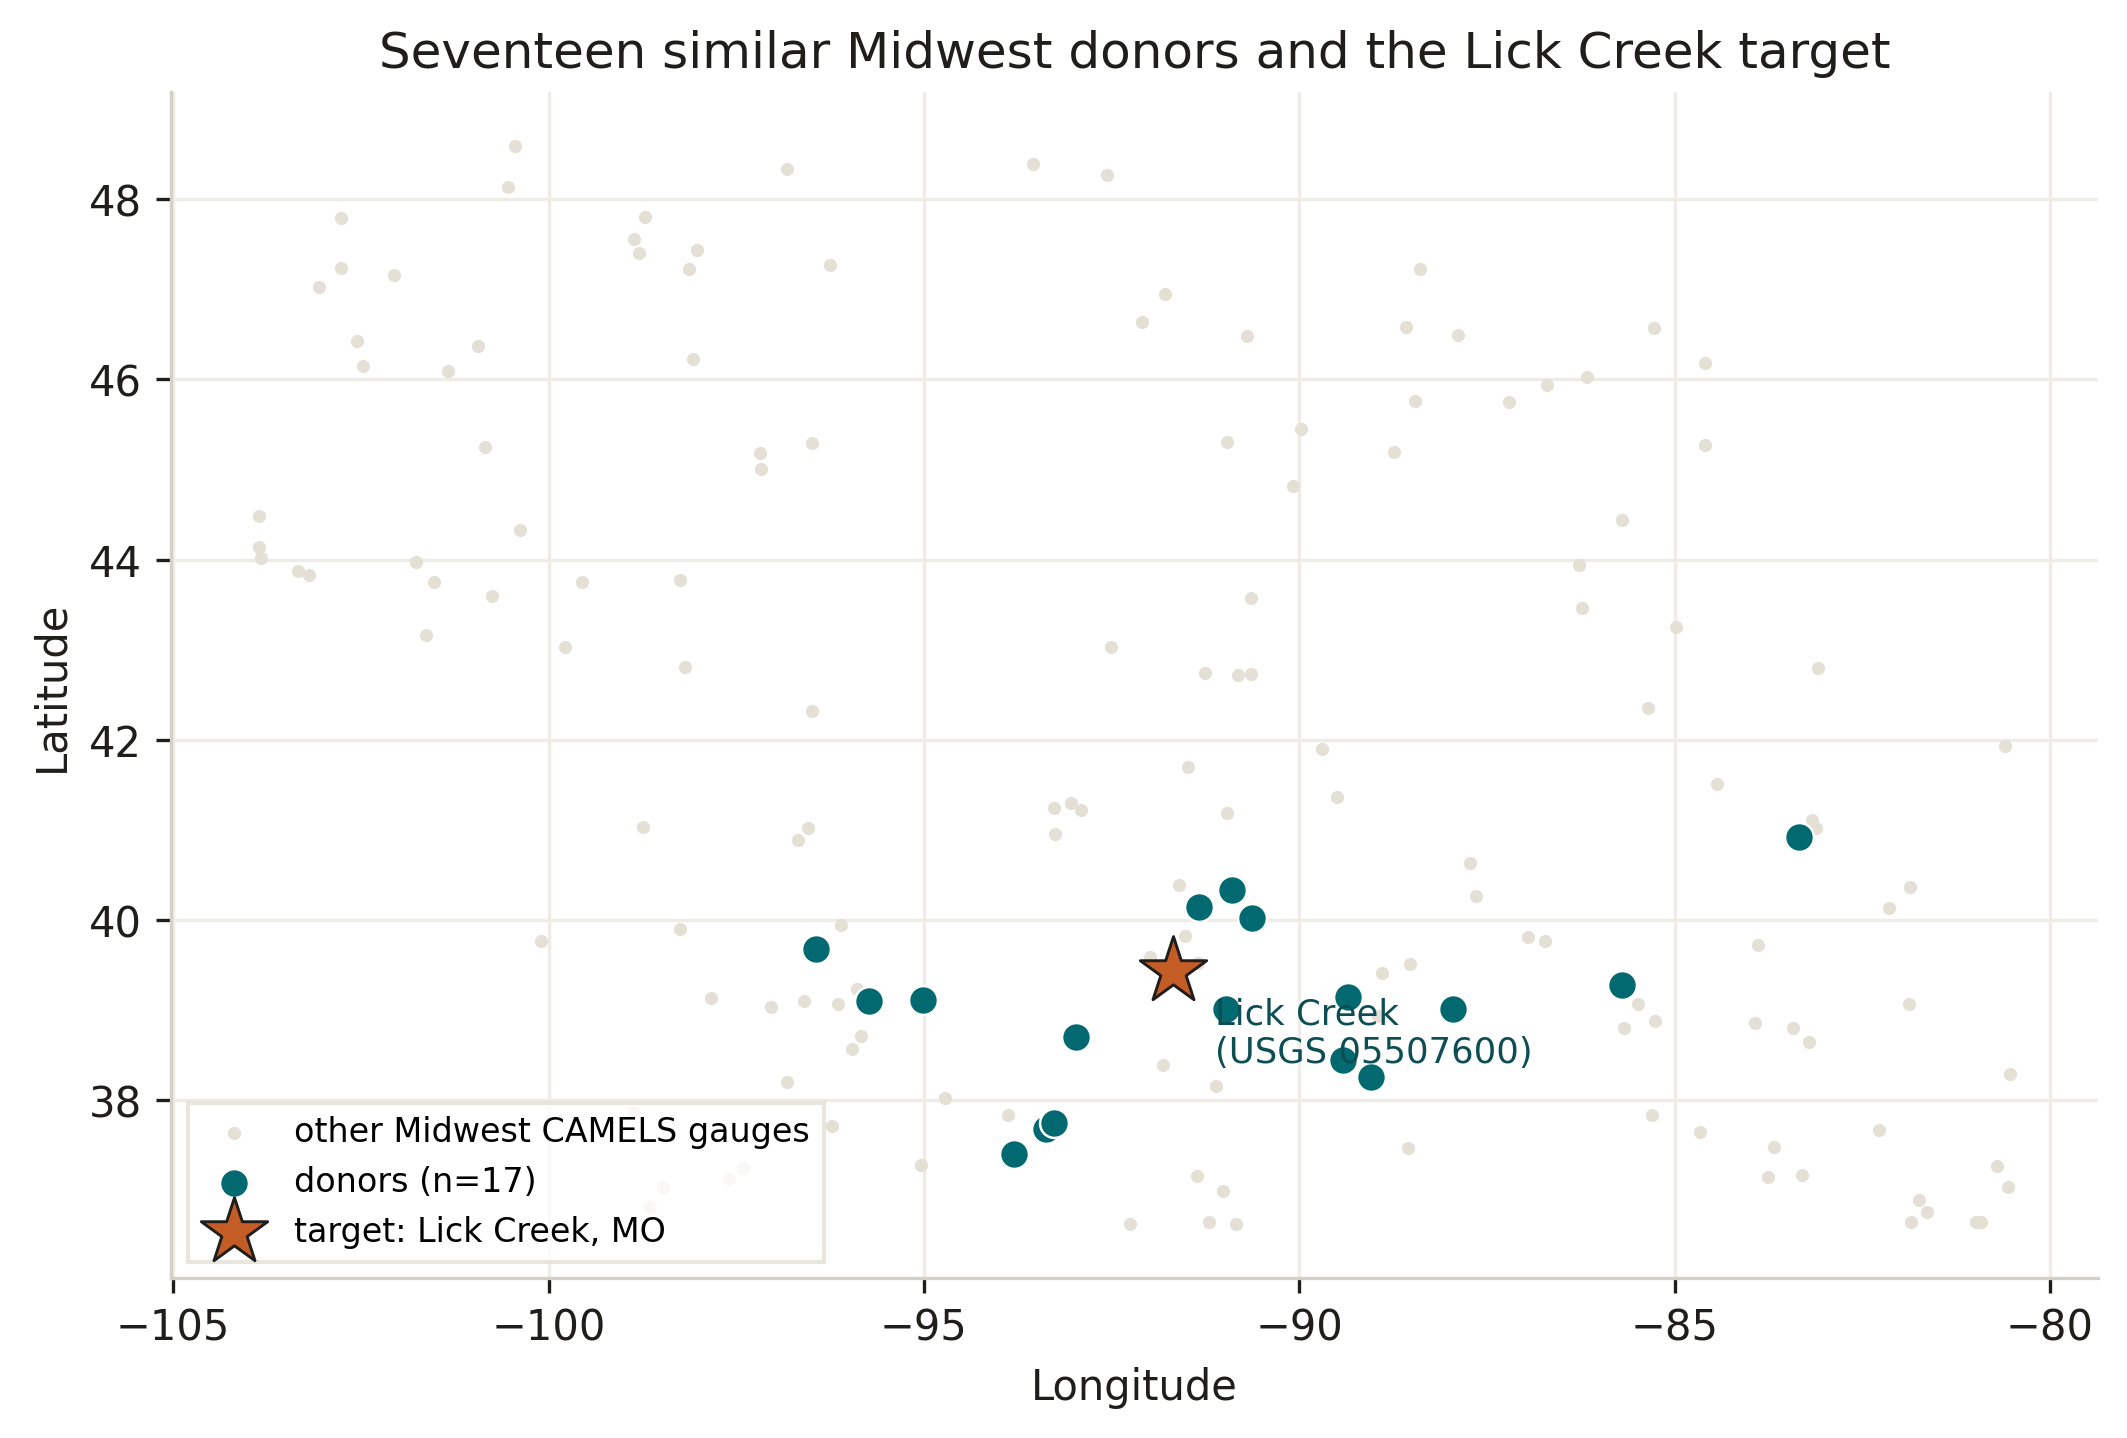
\includegraphics[width=0.88\linewidth]{fig_donor_target_map.png}
  \caption{Seventeen similar Midwest donor gauges and the Lick Creek target.
    Grey points are other CAMELS gauges in the same box; they are context, not
    training data.}
  \label{fig:donors}
\end{figure}

\begin{table}[ht]
  \centering
  \caption{Time periods used for USGS 05507600.}
  \label{tab:periods}
  \small
  \begin{tabular}{@{}llp{5.2cm}@{}}
    \toprule
    \textbf{Period} & \textbf{Dates} & \textbf{Role} \\
    \midrule
    Donor pretrain & Oct.\ 1995--Sep.\ 2008 & Train the regional EA-LSTM \\
    Pretrain validation & Oct.\ 2008--Sep.\ 2010 & Early stopping \\
    Target warmup & Jan.\ 2009--Dec.\ 2010 & Scarce local record (${\sim}$2\,yr) \\
    Target evaluation & 2011--2014 & Fixed-window and walk-forward tests \\
    Threshold history & 1990--2010 & At-site Q5, Q95, Q99 \\
    \bottomrule
  \end{tabular}
\end{table}

\subsection{Model and transfer}

The model is an EA-LSTM: static catchment attributes control the input gate;
weather and memory drive the remaining gates. Hidden size is 128, lookback
\textbf{90} days, dropout 0.4, forget-gate bias $+3.0$. Pretraining runs 10
epochs on the 17 donors. Adaptations compared: zero-shot; Approach~A (output
head only; LSTM frozen); local-from-scratch on the warmup; walk-forward with a
head-only refit every 90 days from 2009-01-01 and online bias correction.
Approach~B was not run here. The scored window is 2011--2014 ($n=1461$ days).

\subsection{Naive baselines and warnings}

Persistence sets $\hat Q(t)=Q(t-1)$. Day-of-year climatology is the mean
observed discharge on that calendar day during warmup 2009--2010 only.
Warnings are a post-process on the walk-forward hydrograph. Labels at date $t$
with lead $L$ are 1 if any day in $[t+1,t+L]$ crosses the threshold. Flood
thresholds are Q95~$=3.26$\,mm\,d$^{-1}$ and Q99~$=16.91$\,mm\,d$^{-1}$.
\textbf{Q5 resolves to $0.0$\,mm\,d$^{-1}$}, so those events are low/zero-flow
days, not a seasonal drought. Original probabilities use a Gaussian residual
and an independence product over the lead window. A second estimator takes the
maximum of the 1-day probabilities in the same window. Metrics: NSE, KGE,
PBIAS, AUC, Brier, BSS against the event base rate, F1 at 0.5 and at the
threshold in $\{0.05,\ldots,0.95\}$ that maximises F1 on the scored window
(diagnostic only).

\section{Results}

\subsection{Continuous streamflow skill}

Table~\ref{tab:midwest_metrics} places transfer above both naive baselines and
the local LSTM. Walk-forward NSE (0.179) is the best continuous score.
Persistence has a high KGE (0.42) because yesterday is correlated with today,
but its NSE is negative ($-0.166$): peak errors on this flashy plains
hydrograph more than eat the variance. Climatology from two years of warmup is
worse (NSE $=-2.34$). Local-from-scratch barely beats a mean forecast
(NSE~$=0.009$). Fine-tuning almost removes volume bias (PBIAS $+4.1\%$).
Absolute NSE is modest next to continental LSTMs; the ranking that answers the
study question is not: \textbf{transfer $\gg$ local}, and transfer beats
persistence on NSE.

\begin{table}[ht]
  \centering
  \caption{Continuous skill at USGS 05507600, 2011--2014 ($n=1461$ days).}
  \label{tab:midwest_metrics}
  \small
  \begin{tabular}{@{}lrrr@{}}
    \toprule
    \textbf{Setting} & \textbf{NSE} & \textbf{KGE} & \textbf{PBIAS (\%)} \\
    \midrule
    Next-day persistence & $-0.166$ & 0.421 & $+1.6$ \\
    Day-of-year climatology (warmup) & $-2.337$ & $-1.486$ & $+223.1$ \\
    Local baseline (from-scratch warmup) & 0.009 & $-0.351$ & $+72.6$ \\
    Zero-shot (pretrained only) & 0.150 & 0.032 & $-37.5$ \\
    Fine-tune, head only (Approach A) & 0.160 & 0.112 & $+4.1$ \\
    Walk-forward (17$\times$ 90-day refits) & 0.179 & 0.161 & $-8.7$ \\
    \bottomrule
  \end{tabular}
\end{table}

\begin{figure}[ht]
  \centering
  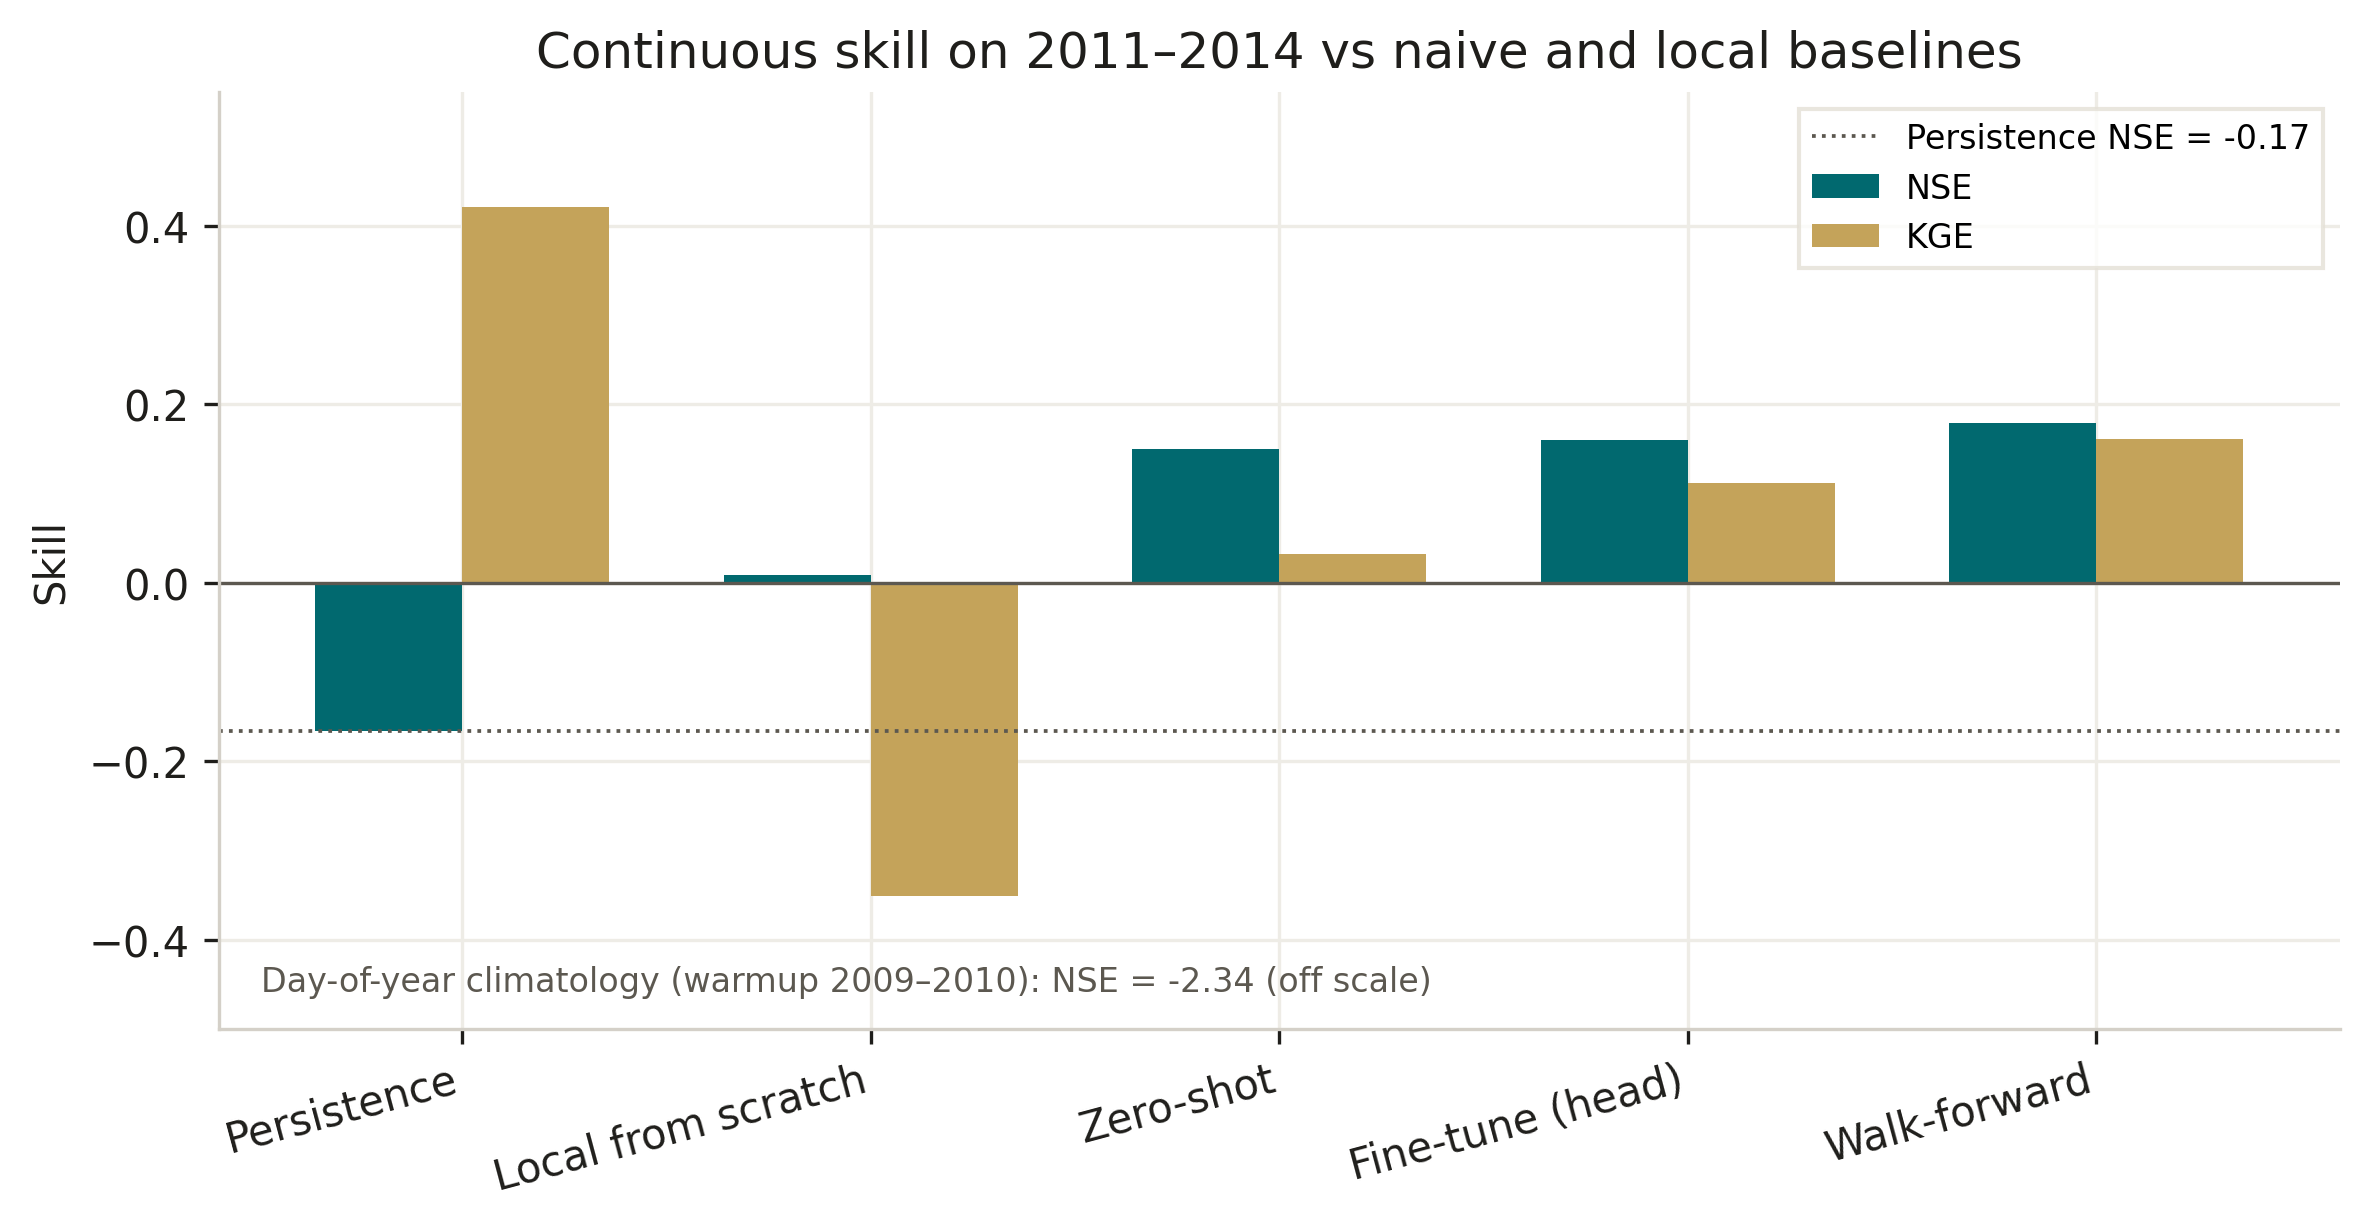
\includegraphics[width=0.92\linewidth]{fig_skill_bars.png}
  \caption{NSE and KGE across settings. Dotted line: persistence NSE.
    Day-of-year climatology (NSE $=-2.34$) is annotated, not forced onto the
    same axis.}
  \label{fig:bars}
\end{figure}

\begin{figure}[ht]
  \centering
  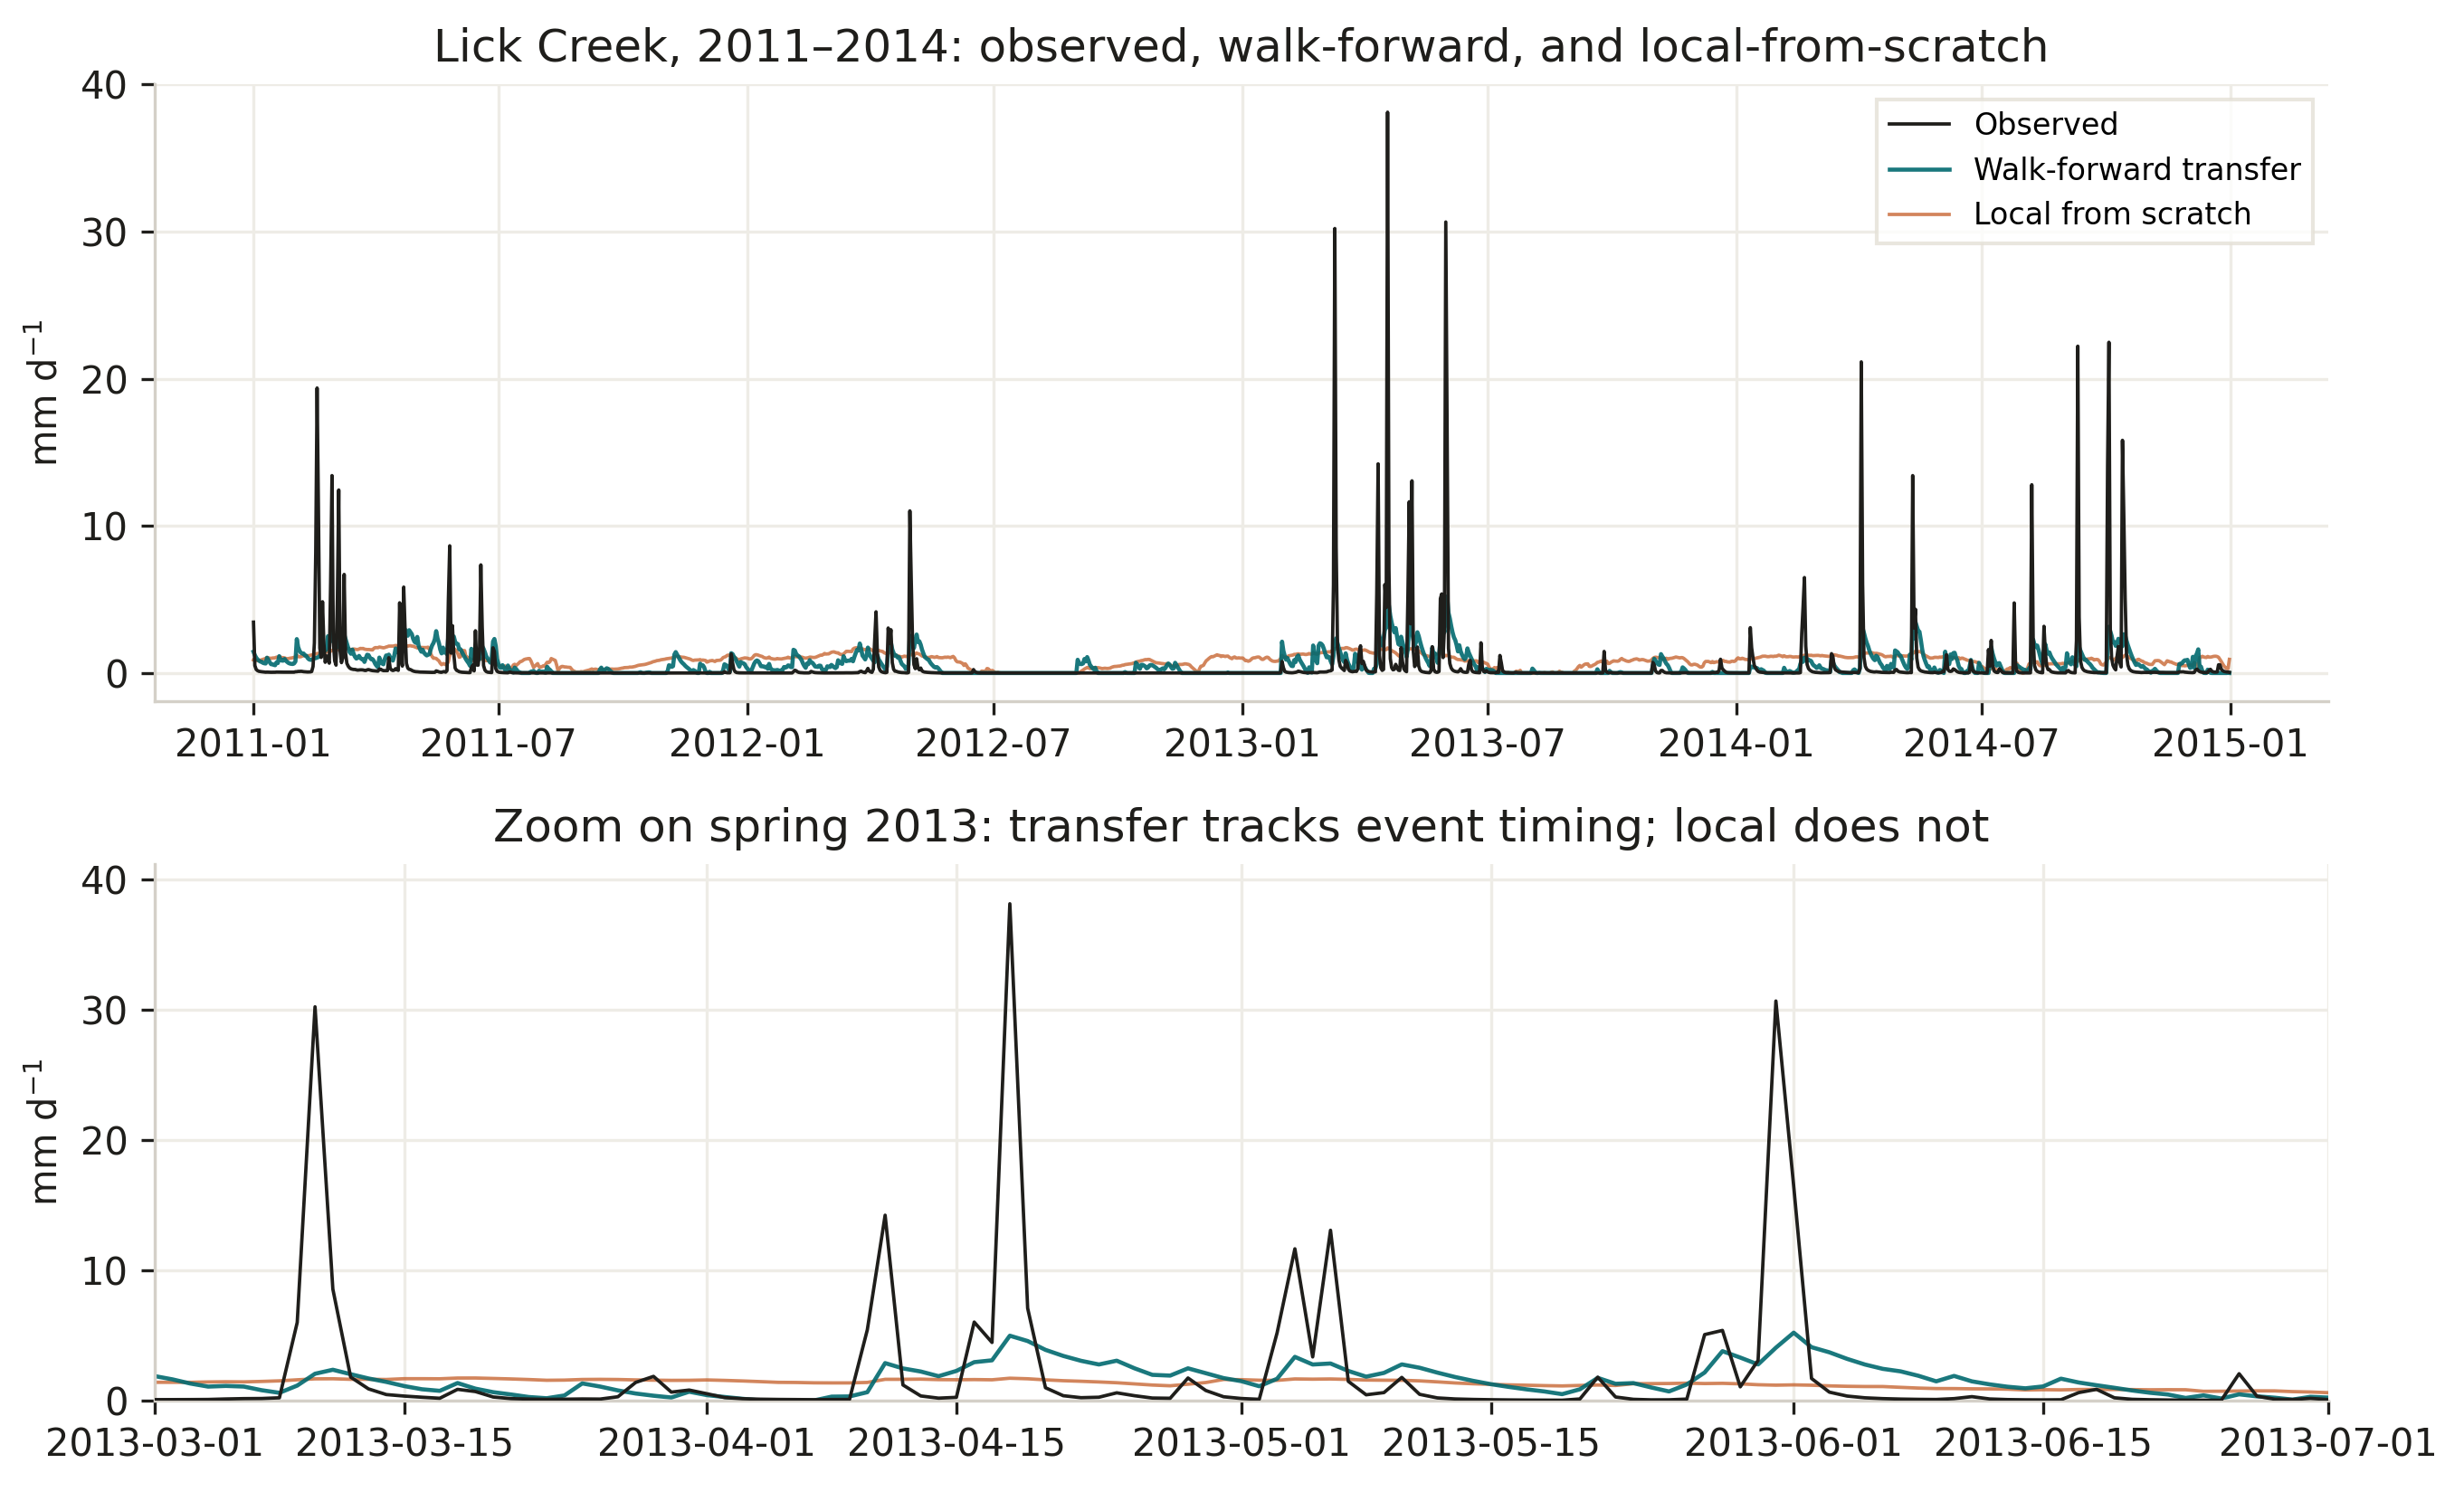
\includegraphics[width=0.95\linewidth]{fig_hydrograph_2011_2014.png}
  \caption{Observed discharge versus walk-forward transfer and
    local-from-scratch. Transfer follows event timing; the local model does
    not. Predictions clipped at zero for display.}
  \label{fig:hydro}
\end{figure}

\subsection{Early-warning scores and calibration}

Flood Q95 discrimination is strong at every lead (AUC 0.908--0.922). Raw Brier
scores still look as if skill collapses from 0.094 (1-day) to 0.693 (7-day).
BSS against the base rate is negative for the independence product:
mean 1-day probability is 0.29 while the event rate is 0.034, and the 7-day
product has mean probability 0.89. Ranking is intact; calibration is not.
Replacing the product with a window-max of 1-day probabilities cuts 3-day
Brier from 0.374 to 0.105 and 7-day Brier from 0.693 to 0.121. F1 at 0.5 is
the wrong operating point; a threshold sweep raises 1-day F1 from 0.286 to
0.452 at probability 0.45 (Table~\ref{tab:midwest_ews};
Figure~\ref{fig:reliab}).

\begin{table}[ht]
  \centering
  \caption{Walk-forward warning scores. Prod.\ = independence product;
    max = window-max of 1-day probabilities. F1* is the best F1 on a
    0.05--0.95 sweep (diagnostic). Q5 $=0$\,mm\,d$^{-1}$ (low/zero flow).}
  \label{tab:midwest_ews}
  \small
  \renewcommand{\arraystretch}{1.05}
  \begin{tabular}{@{}llrrrrrrr@{}}
    \toprule
    \textbf{Event} & \textbf{Lead} & \textbf{AUC} & \textbf{Brier$_{\mathrm{p}}$} & \textbf{BSS$_{\mathrm{p}}$} & \textbf{Brier$_{\mathrm{m}}$} & \textbf{BSS$_{\mathrm{m}}$} & \textbf{F1@0.5} & \textbf{F1*} \\
    \midrule
    Flood Q95 & 1\,d & 0.922 & 0.094 & $-1.90$ & 0.094 & $-1.90$ & 0.286 & 0.452 \\
    Flood Q95 & 3\,d & 0.914 & 0.374 & $-4.87$ & 0.105 & $-0.65$ & 0.133 & 0.500 \\
    Flood Q95 & 7\,d & 0.908 & 0.693 & $-5.45$ & 0.121 & $-0.13$ & 0.219 & 0.621 \\
    Flood Q99 & 1\,d & 0.950 & 0.005 & --- & 0.005 & --- & --- & --- \\
    Low/zero flow (Q5) & 1\,d & 0.805 & 0.214 & $-0.74$ & 0.214 & $-0.74$ & 0.410 & 0.419 \\
    \bottomrule
  \end{tabular}
\end{table}

\begin{figure}[ht]
  \centering
  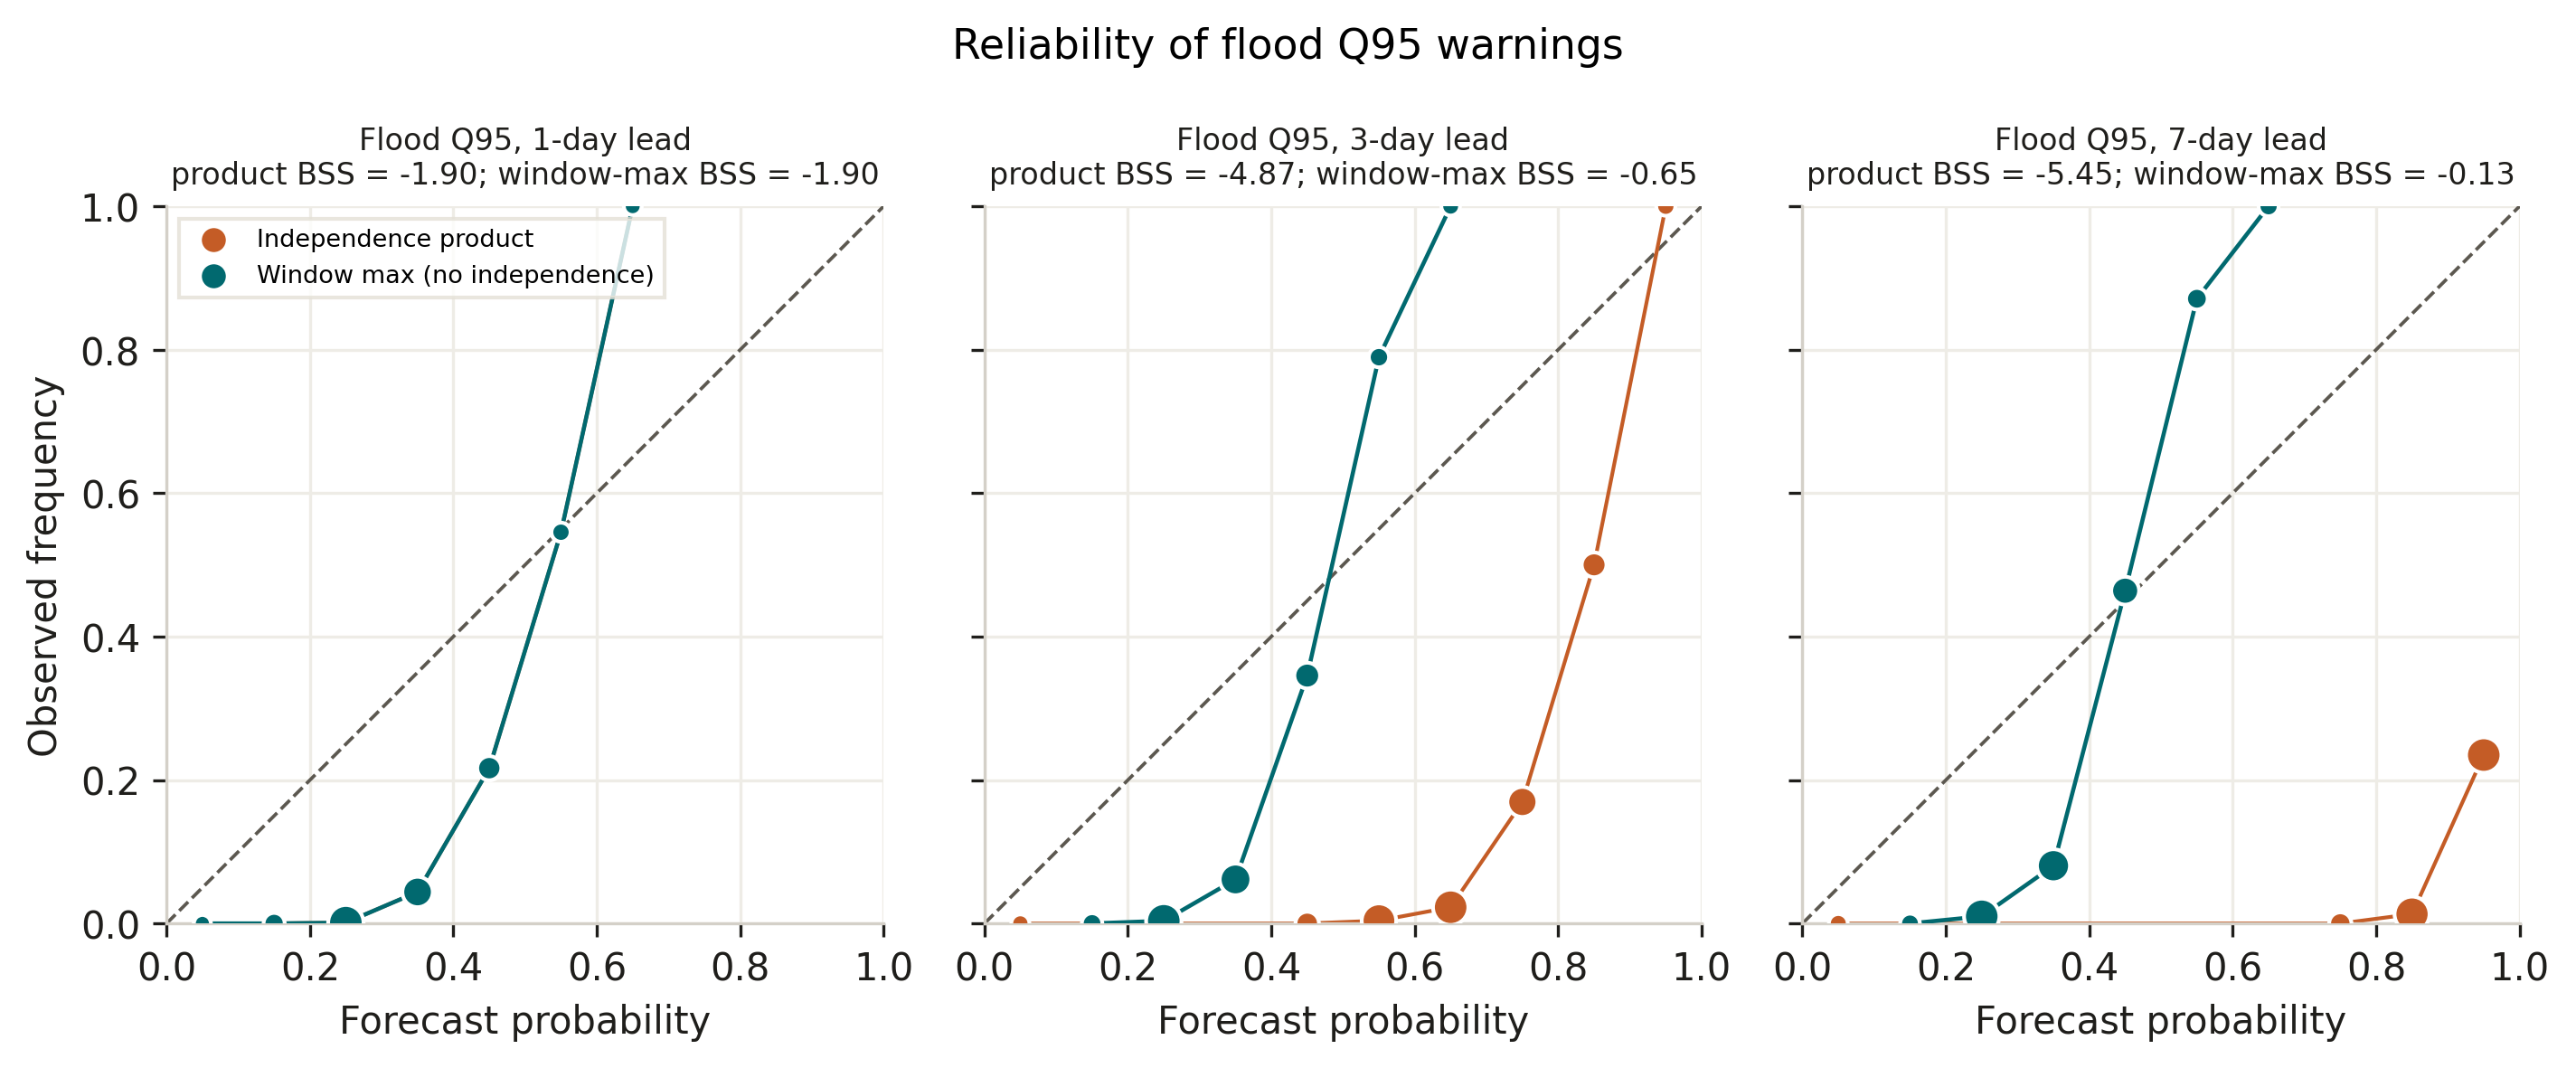
\includegraphics[width=0.98\linewidth]{fig_reliability_q95.png}
  \caption{Reliability of flood Q95 warnings. Coral: independence product.
    Teal: window-max of 1-day probabilities.}
  \label{fig:reliab}
\end{figure}

\subsection{SHAP drivers}

GradientExplainer ranks precipitation first, then vapor pressure, shortwave
radiation, day length, $T_\mathrm{min}$, and $T_\mathrm{max}$
(Table~\ref{tab:midwest_shap}). Static attributes have mean $|$SHAP$|=0$ in
this single-basin explanation because they do not vary within one gauge.

\begin{table}[ht]
  \centering
  \caption{Top SHAP drivers for USGS 05507600.}
  \label{tab:midwest_shap}
  \small
  \begin{tabular}{@{}lr@{}}
    \toprule
    \textbf{Feature} & \textbf{Mean $|$SHAP$|$} \\
    \midrule
    Precipitation (mm/day) & 0.0097 \\
    Vapor pressure (Pa) & 0.0055 \\
    Shortwave radiation (W/m$^2$) & 0.0052 \\
    Day length (s) & 0.0041 \\
    $T_\mathrm{min}$ ($^\circ$C) & 0.0036 \\
    $T_\mathrm{max}$ ($^\circ$C) & 0.0035 \\
    Static catchment attributes (all) & 0.0000 \\
    \bottomrule
  \end{tabular}
\end{table}

\subsection{How few donors? A negative result}

Table~\ref{tab:opt_metrics} keeps the donor-pruning comparison. Cutting 17
similar donors to 8, with Tmin/Tmax unchanged, lowers walk-forward NSE from
0.179 to 0.138. Combining pruning with mean daily temperature and a three-seed
average recovers some of that loss (NSE 0.165) but still does not beat the
17-donor run. \textbf{The third row of Table~\ref{tab:opt_metrics} changes
three variables at once} (donor count, temperature features, and multi-seed
averaging) and should not be read as a single-factor effect. Forget-gate bias
$+3.0$ is already the default in every row. Transfer still beats
local-from-scratch after pruning.

\begin{table}[ht]
  \centering
  \caption{Sensitivity to donor pruning (USGS 05507600, 2011--2014 NSE).
    The third row changes donor count, temperature inputs, and seed averaging
    together.}
  \label{tab:opt_metrics}
  \small
  \begin{tabular}{@{}lrrrr@{}}
    \toprule
    \textbf{Setting} & \textbf{Donors} & \textbf{FT} & \textbf{Local} & \textbf{WF} \\
    \midrule
    Tmin+Tmax, seed 42 & 17 & 0.160 & 0.009 & 0.179 \\
    Tmin+Tmax, seed 42 & 8 & 0.113 & 0.009 & 0.138 \\
    Mean $T$, 3-seed average & 8 & 0.133 & $-0.097$ & 0.165 \\
    \bottomrule
  \end{tabular}
\end{table}

\begin{figure}[ht]
  \centering
  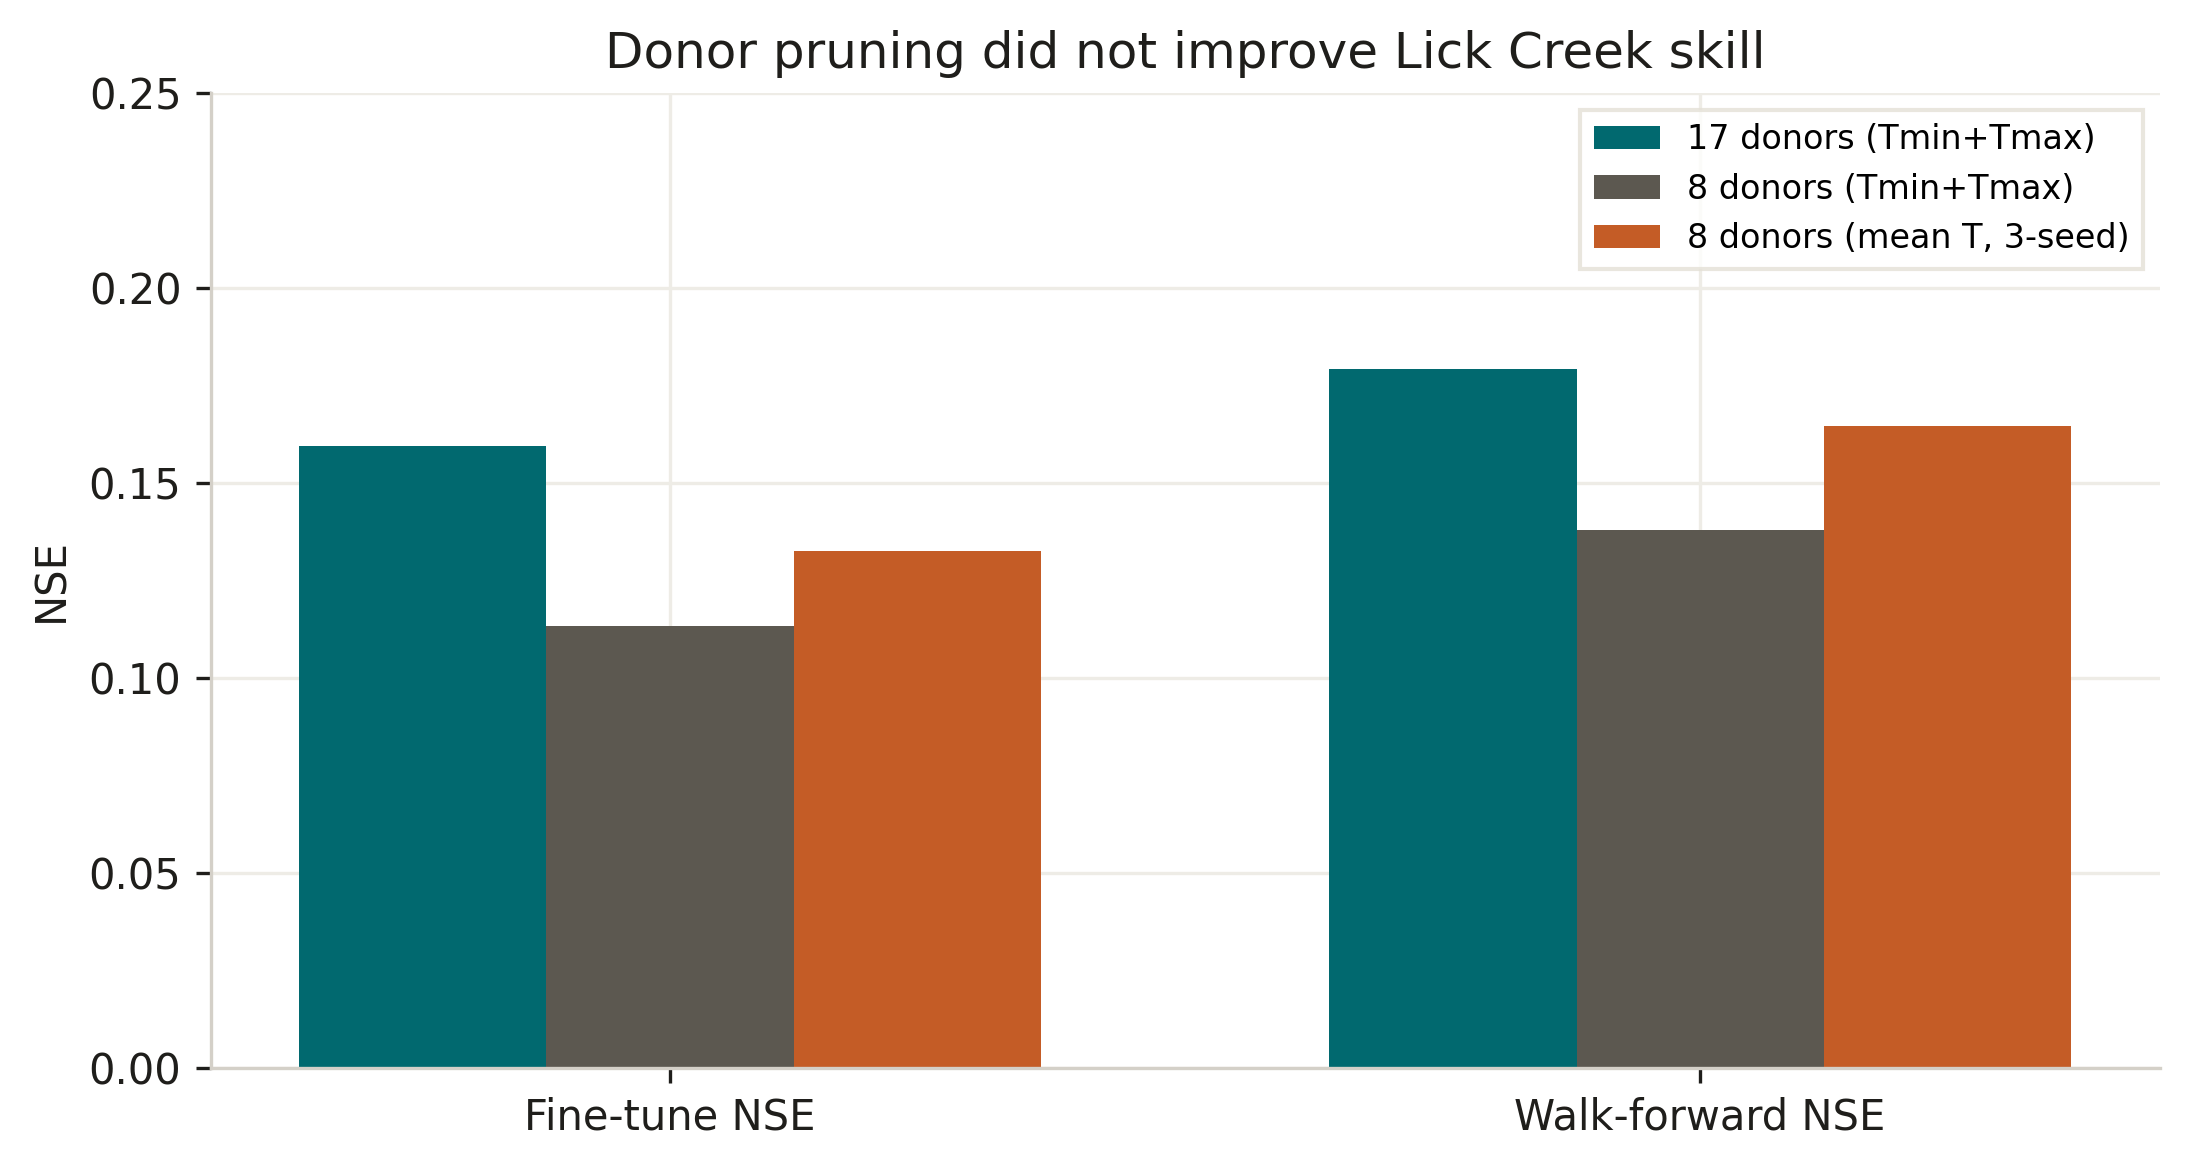
\includegraphics[width=0.82\linewidth]{fig_donor_pruning.png}
  \caption{Seventeen similar donors outperform an 8-donor pool on both
    fine-tune and walk-forward NSE.}
  \label{fig:prune}
\end{figure}

\section{Discussion and conclusion}

This is a one-basin Midwest study on commodity hardware. It does not estimate
continental CAMELS skill or snowmelt-regime transfer. What it does estimate,
with a full 2011--2014 evaluation, is whether a small similar-donor prior beats
local training and naive baselines when local data are scarce. It does.

Warnings are hindcast post-processing of daily flow. F1* uses the same window
it scores. Daily 1-day probabilities remain overconfident (BSS $=-1.90$) even
before compounding; recalibrating that 1-day probability is future work.

With two years of local discharge and a laptop, seventeen similar Midwest
donors are enough for regional transfer to beat both a local LSTM and next-day
persistence on NSE. Eight donors are worse, not better. Flood Q95 warnings
discriminate well; the ugly raw Brier numbers at long leads are mostly an
independence assumption, not a collapse of ranking skill.

\vspace{0.6em}
{\small
Midwest run: \texttt{python scripts/run\_midwest\_mini.py}.
Baselines and figures: \texttt{python scripts/analysis/poster\_from\_csvs.py}.
Word manuscript: \texttt{python scripts/paper/build\_short\_paper\_docx.py}.
}

\end{document}
